\documentclass[a4paper,12pt,landscape]{article}
\usepackage{multicol}
\usepackage{calc}
\usepackage{ifthen}
\usepackage[a4paper, landscape]{geometry}
\usepackage{amsmath,amsthm,amsfonts,amssymb}
\usepackage{color,graphicx,overpic}
\usepackage{hyperref}
\usepackage{tabulary}
\usepackage{soul} %for highlight
\usepackage{xcolor} %color definition
\usepackage{sectsty} %change section color
\usepackage{tabulary} % better table

% type codes
\usepackage{listings} 
\usepackage{xcolor}

\definecolor{codegreen}{rgb}{0,0.6,0}
\definecolor{codegray}{rgb}{0.5,0.5,0.5}
\definecolor{codepurple}{rgb}{0.58,0,0.82}
\definecolor{backcolour}{rgb}{0.95,0.95,0.92}

\lstdefinestyle{mystyle}{
    backgroundcolor=\color{backcolour},   
    commentstyle=\color{codegreen},
    keywordstyle=\color{magenta},
    numberstyle=\tiny\color{codegray},
    stringstyle=\color{codepurple},
    basicstyle=\ttfamily\footnotesize,
    breakatwhitespace=false,         
    breaklines=false,                 
    captionpos=b,                    
    keepspaces=false,                 
    numbers=left,                    
    numbersep=5pt,                  
    showspaces=false,                
    showstringspaces=false,
    showtabs=false,                  
    tabsize=2
}

\lstset{style=mystyle}

\pdfinfo{
  /Title (ST3247 Simulation.pdf)
  /Creator (Ling)
  /Subject (Simulation)}

% This sets page margins to .5 inch if using letter paper, and to 1cm
% if using A4 paper. (This probably isn't strictly necessary.)
% If using another size paper, use default 1cm margins.
\ifthenelse{\lengthtest { \paperwidth = 11in}}
    { \geometry{top=.5in,left=.5in,right=.5in,bottom=.5in} }
    {\ifthenelse{ \lengthtest{ \paperwidth = 297mm}}
        {\geometry{top=.5cm,left=.5cm,right=.5cm,bottom=.5cm} }
        {\geometry{top=.5cm,left=.5cm,right=.5cm,bottom=.5cm} }
    }

% Turn off header and footer
\pagestyle{empty}

% Redefine section commands to use less space
\makeatletter
\renewcommand{\section}{\@startsection{section}{1}{0mm}%
                                {-1ex plus -.5ex minus -.2ex}%
                                {0.5ex plus .2ex}%x
                                {\normalfont\large\bfseries\color{red}}}
\renewcommand{\subsection}{\@startsection{subsection}{2}{0mm}%
                                {-1explus -.5ex minus -.2ex}%
                                {0.5ex plus .2ex}%
                                {\normalfont\normalsize\bfseries\color{blue}}}
\renewcommand{\subsubsection}{\@startsection{subsubsection}{3}{0mm}%
                                {-1ex plus -.5ex minus -.2ex}%
                                {1ex plus .2ex}%
                                {\normalfont\small\bfseries\color{violet}}}
\makeatother

% Define BibTeX command
\def\BibTeX{{\rm B\kern-.05em{\sc i\kern-.025em b}\kern-.08em
    T\kern-.1667em\lower.7ex\hbox{E}\kern-.125emX}}

% Don't print section numbers
\setcounter{secnumdepth}{0}


\setlength{\parindent}{0pt}
\setlength{\parskip}{0pt plus 0.5ex}

%My Environments
\newtheorem{example}[section]{Example}
% -----------------------------------------------------------------------

\begin{document}
\raggedright
\footnotesize
\begin{multicols}{3}


% multicol parameters
% These lengths are set only within the two main columns
\setlength{\columnseprule}{0.25pt}
\setlength{\premulticols}{1pt}
\setlength{\postmulticols}{1pt}
\setlength{\multicolsep}{1pt}
\setlength{\columnsep}{2pt}

\begin{center}
     \Large{\underline{ST3247 Simulation}} \\
     {Lingjie, \today}
\end{center}

\begin{section}{R programming}

	\begin{subsection}{Common functions}
		\begin{tabulary}{\linewidth}{l @{ : }  L}
			remainder & \%\% \\
			matrix multiplication & \%*\% \\
			rounding & floor, ceiling, round, signif \\
			load R commands & source(filename, echo=TRUE) \\
			set seed & set.seed(1234) \\
			vectorise function & Vectorize(fn) \\
			apply & sapply(X, fn, *params) \\
			& apply(X, 1, fn) \\ &1 := row, 2 := col \\
			generate sample & rxxxx \\
			pdf $P(X=x), f_X$ & dxxxx \\
			cdf $P(X\leq x), F_X$ & pxxxx \\
			cdf quantile $F^{-1}(x)$ & qxxxx \\
		\end{tabulary}
	\end{subsection}
\end{section}

\begin{section}{\small{Probability and Math Stat Background}}

	\begin{subsection}{Important knowledge}
		\begin{tabulary}{\linewidth}{l L}
			Law of Total Probability  \\$P(X \in A)$ \\ 
			= $\sum_{i=1}^nP(X \in A, Y \in B_i)$ \\
			 = $\sum_{i=1}^n P(X\in A|Y \in B_i)P(Y \in B_i)$ \\
			 Indicator function: $I(a < x < b)$ \\
			 Mode of distribution\\
			 Discrete: $i$ s.t. $p_i \geq p_j~\forall j \neq i$\\
			 Continuous: $x$ s.t. $f(x) \geq f(w)~\forall x\neq w$\\
			 Conditional Expectation: \\ 
             $E(X|Y = y) = \int xf_{x|y}(x|y) dx = \frac{\int xf_{x,y}(x, y) dx}{\int f_Y(y) dx}$\\
			 and $E(X) = E(E(X|Y))$ \\
			 Conditional Variance: \\
			 $Var(X) = E(Var(X|Y)) + Var(E(X|Y))$ \\
			 $Var(X) \geq Var(E(X|Y))$
		\end{tabulary}
	\end{subsection}

	\begin{subsection}{Computing RV pmf Recursively}
		\begin{subsubsection}{Binomial}
			\begin{tabulary}{\linewidth}{l @{ = } l}
				$P(X = x+1)$  & $ \frac{n!}{(n-x-1)!(x+1)!}p^{x+1}(1-p)^{n-x-1}$ \\
				& $\frac{n!(n-x)}{(n-x)!x!(x+1)}p^x(1-p)^{n-x}\frac{p}{1-p}$ \\
				& $\frac{n-x}{x+1}\frac{p}{1-p}P(X=x)$
			\end{tabulary}
		\end{subsubsection}
		
		\begin{subsubsection}{Poisson}
			For $x\geq 0$ \\
			\begin{tabulary}{\linewidth}{l @{ = } l}
				$P(X = x+1)$ & $e^{-\lambda}\frac{\lambda^{x+1}}{(x+1)!}$ \\
				& $\frac{\lambda}{x+1}e^{-\lambda}\frac{\lambda^x}{x!}$ \\
				& $\frac{\lambda}{x+1}P(X=x)$
			\end{tabulary}
		\end{subsubsection}
	\end{subsection}

	\begin{subsection}{Solving Min Max RV}
		Let $Y \sim min(X_1, X_2)$ $X_1, X_2$ are independent\\ 
		$P(Y \leq y) = P(min(X_1, X_2) \leq y) = 1 - P(min(X_1, X_2) > y)$ \\
		$= 1 - P(X_1 > y, X_2 > y) = 1 - P(X_1 > y)P(X_2 > y)$
		
		Let $Y \sim max(X_1, X_2)$ $X_1, X_2$ are independent\\ 
		$P(Y \leq y) = P(max(X_1, X_2) \leq y)$ \\
		$= P(X_1 \leq y, X_2 \leq y) = P(X_1 \leq y)P(X_2 \leq y)$
	\end{subsection}

	\begin{subsection}{Uniform Distribution}
		\begin{tabulary}{\linewidth}{l @{ : } L}
			pdf & $f(x) = \frac{1}{b-a}I(a\leq x \leq b)$ \\
			cdf & $F(x) = \frac{x-a}{b-a}$ \\
			$E(X)$ & $\frac{b+a}{2}$ \\
			$Var(X)$ & $\frac{(b-a)^2}{12}$
		\end{tabulary}
	\end{subsection}

    \begin{subsection}{\colorbox{pink}{Poisson Process}}
		$N(t) := $ number of events in the time interval $[0, t]$ \\
		$N(t+s) :=$ number of events in the time interval $[0, t+s]$ \\
		$N(t+s) - N(t) :=$ num of events in the time interval $[t, t+s]$ \\
		$m(t) :=$ the area under the intensity function from $0$ to $t$ \\
		$m(t+s) - m(t) :=$ the area under the intensity function from $t$ to $t+s$ \\
		process is defined as Poisson process with rate $\lambda, \lambda > 0$ if \\
		\begin{enumerate}
			\item $N(0) = 0$ \\
				$\Rightarrow$ nothing happened before time 0
			\item Number of events occurring in disjoint time intervals are independent \\
				$\Rightarrow$ independent increments assumption\\ $\Rightarrow$ e.g. $N(t)$ is independent of $N(t+s) - N(t)$
			\item Distribution of number of events only depend on length of interval, not location \\
				$\Rightarrow$ stationary increment assumption \\
				$\Rightarrow$ distribution of event across every interval of time is the same
			\item $\lim_{h\rightarrow 0} \frac{P(N(h) = 1}{h} = \lambda $ \\
				$\Rightarrow$ within a small interval of length h, the probability of one event is approximately $\lambda h$
			\item $\lim_{h\rightarrow 0} \frac{P(N(h) \geq 2)}{h} = 0$ \\
				$\Rightarrow$ within a small interval of length h, the probability of two or more events is approximately 0
		\end{enumerate}
		Therefore, $N(t) \sim Pois(\lambda t)$
		
		\begin{subsubsection}{Non-homogeneous Poisson Process}
			$N(t) :=$ number of events by time $t$\\
			$N(t)$ is a non-homogenous Poisson process with intensity function $\lambda (t)$ if \\
			(same condition as Poisson Process except) \\
			\begin{enumerate}
				\item $\lim_{h\rightarrow p}P($exactly 1 event between $t$ and $t+h)/h=\lambda (t)$
			\end{enumerate}
			$N(t+s) - N(t) = Pois(m(t+s) - m(t))$
		\end{subsubsection}

        \subsection{Mean value function}
        \hl{Definition 1 (Mean Value Function)}
        \begin{align*}
            m(t) = \int_0^t \lambda(s) ds, t\geq0
        \end{align*}
        $\lambda(t):=$ intensity at time $t$, indicates how likely it is that event will occur around time $t$.\\
        $N(t+s) - N(t) = Pois\left( m(t+s)-m(t)  \right)$
		
	\end{subsection}

\end{section}

\begin{section}{Pseudo-Random Number Generation}
	\begin{subsection}{Types of PRNGs}
		\begin{subsubsection}{Linear Congruential Generators}
			Pseudo-code for LCG
			\begin{enumerate}
				\item Set $Z_0$
				\item For $i=1$ to $n$:
					\subitem 1. Set $Z_i = (aZ_{i-1} +c)$ mod $m$
					\subitem 2. Set $U_i = Z_i /m$
			\end{enumerate}
			
			Obtaining Full Period
			\begin{enumerate}
				\item Only positive integer that divides both $m$ and $c$ is 1
				\item If $q$ is prime num that divides $m$, then $q$ divides $a-1$
				\item If $4$ divides $m$, then $4$ divides $a-1$
			\end{enumerate}
		\end{subsubsection}
		
		\begin{subsubsection}{PRNG in R}
			shift register with period $2^{19937} -1$
		\end{subsubsection}
	\end{subsection}
	
	\begin{subsection}{Statistical Tests for PRNGs}
		\begin{subsubsection}{Frequency Test: Check for Uniformity}
			check: if $U_i$ appear to be evenly distributed between 0 and 1
		\end{subsubsection}
		
		\begin{subsubsection}{Correlation Test: Check for Autocorrelation}
			check: no correlation at lag $j$ for all $j$
		\end{subsubsection}
	\end{subsection}
\end{section}

\section{Discrete Random Variable Generation}
	\textbf{Objective}: Given pmf, generate random variable\\
	\textbf{Constraint}: \\
    1. $E(N)$, 2. num of $Unif[0,1]$, 3. storage space

	\begin{tabulary}{\linewidth}{| L | c | c | c | C |}
		\hline
		 Algo & No. iter & No. RVs & Storage & \scriptsize Infinite support?\\
		\hline
		\hline
		\scriptsize Seq. Inversion & \scriptsize$E(X)+1$ & 1 & - & Y\\
		\hline
		\scriptsize Ordered. Inversion & \scriptsize$< E(X) +1$ & 1 & \scriptsize Variable & Y\\
		\hline
		\scriptsize Truncation & 1 & 1 & - & Y\\
		\hline
		\scriptsize Rejection & $\approx c$ & $\approx 2c$ & - & Y\\
		\hline
		\scriptsize Table & 1 & 1 & M & N\\
		\hline
		\scriptsize Alias & 2 & 2 & 3(K-1) & N\\
		\hline
	\end{tabulary}

	\subsection{Inversion Method}
	
		\subsubsection{Sequential Inversion}
			\hl{Algorithm 1 [Sequential Inversion]}
			\begin{enumerate}
				\item Generate $U \sim Unif[0, 1]$
				\item Set $X = 0, S = p_0 \Rightarrow P(X=0)=p_0$
				\item While $U > S$, do
					\subitem{3.1} $X = X + 1$
					\subitem{3.2} $S = S + p_x$
				\item Return $X$
			\end{enumerate}
		
		\hl{R Implementation [Poisson]}
		\begin{lstlisting}[language=R]
U <- runif(n=1, min=0, max=1) #cdf
X <- 0; S <- exp(-lambda)) #P(X=0)
while(U > S){
	X <- X + 1
	S <- S + exp(-lambda)*(lambda^X)/
			factorial(X)
}
print(X)
			\end{lstlisting}
		
		\hl{Expected Iterations}
		\begin{align*}
			E(N) =& 1P(X=0)+2P(X=1)+3P(X=2)+\cdots\\
			=&0P(X=0)+1P(X=0)+2P(X=1)+3P(X=2)\cdots\\
			+&P(X=0)+P(X=1)+P(X=2)+P(X=3)+\cdots\\
			=&E(X)+1
		\end{align*}
		
		\subsubsection{Ordered Inversion}
		Improved Inversion method by checking the largest interval first
		
		\hl{Algorithm 2 [Ordered Inversion]}
		\begin{enumerate}
			\item Set-up Stage:
				\subitem{1.1} Sort $p_i$'s (decreasing)
				\subitem{1.2} $Y$ := indices of the sorted $p_i$'s
				\subitem{1.3} $q_i$ := to be pmf of sorted $p_i$'s
			\item Generation Stage:
				\subitem{2.1} Generate Z from $q_i$ (algo 1)
				\subitem{2.2} Return X = Y[Z+1]
		\end{enumerate}
		\hl{R Implementation [discrete pmf]}
		$X \in \left(p_0=0.2,~ p_1=0.55,~ p_2=0.25\right)$
		\begin{lstlisting}[language=R]
X <- c(0.2, 0.55, 0.25)
###############
# Set-up Stage 
###############
Q <- sort(X, decreasing=TRUE)
#Q = (0.55, 0.25, 0.2)
Y <- c(1, 2, 0) # stored index
#Y adjust with support (start = 1 or 0)
##################
# Generation Stage
##################
U <- runif(n=1, min=0, max=1) #cdf
Z <- 0; S <- Q[1] #P(Q=0)
while(U>S){
  Z <- Z+1
  S <- S+Q[Z+1]
}
Y[Z+1] #generated X
		\end{lstlisting}
		
		\hl{Expected Iterations}
		\begin{align*}
			E(N1) &= E(X) + 1 = 2.05\\
			E(N2) &= [0(0.55)+1(0.25)+2(0.2)]+1=1.65
		\end{align*}
		
		\subsubsection{Truncation of a Related Continuous cdf}

		Required steps
		\begin{itemize}
			\item Identify $G(x)$ by setting $G(i+1)=F(i)$
			\item Show $\frac{dG}{dx}>0 $ (mono increasing) and $0\leq G \leq 1$
			\item G(0) = 0
                \subitem Note: if support starts from 1, check $G(1)=0$
			\item find $G^{-1}(U)$
		\end{itemize}

		\hl{Algorithm 3 [Inversion by Truncation]}
		\begin{enumerate}
			\item Generate $U\sim Unif[0, 1]$
			\item Set $X = \lfloor G^{-1}(U)) \rfloor$
			\item Return X
		\end{enumerate}
	
		\hl{R Implementation [discrete uniform]}\\
		generate $X\sim uniform(0, K-1)$\\
		$F(i) = \sum_{j=0}^i\frac{1}{K}=\frac{i+1}{K}$\\
		$G(i+1) = \frac{i+1}{K} \Rightarrow G(x)=\frac{x}{K}$\\
		$\because G^{-1}(U) = KU \therefore X = \lfloor{KU}\rfloor $
		\begin{lstlisting}[language=R]
U <- runif(n=1) # continuous uniform
X <- floor(K*U)
		\end{lstlisting}
		Note: if $Y\sim uniform(1, K) \Rightarrow Y = X + 1$
		
		\hl{R Implementation [geometric]}\\
		$X\sim Geo(p), q:=1-p$\\
		$P(X=i)=p(1-p)^{i-1}=(1-q)q^{i-1}=q^{i-1}-q^i, i\geq 1$\\
		$F(i)=\sum_{j=1}^iP(X=j)=1-q^i$ (oscillating sum)
		$G(i+1)=F(i)=1-q^i \Rightarrow G(x) = 1-q^{x-1}$\\
		$\because G^{-1}(U) = 1 + \frac{\log(1-U)}{\log q} \therefore X = \lfloor 1 + \frac{\log(1-U)}{\log q} \rfloor$
		\begin{lstlisting}[language=R]
U <- runif(1)
X <- floor(1+log(1-U)/log(q))
		\end{lstlisting}

		\subsubsection{R Implementation [Random Permutation]}
		\hl{Algorithm 4 [Generating Random Permutation]}\\
		Let $P_1P_2\cdots P_n$ be any permutation of the num $\{1,2, \cdots, n\}$
		\begin{enumerate}
			\item Set k=n
			\item Generate $Z \sim Unif(1, 2, \cdots, k)$
			\item Interchange $P_z$ and $P_k$
			\item Update $k = k - 1$
			\item if $k>1$, return to step 2
			\item Return the final permutation $P_1P_2\cdots P_n$
		\end{enumerate}
		\begin{lstlisting}[language=R]
P <- 1:n # ordered numbers
k <- n
while(k>1){
U <- runif(n=1)
z <- floor(k*U) + 1 #discrete unif(1, k)
Pz <- P[z]; Pk <- P[k]
P[k] <- Pz; P[z] <- Pk # interchange value
k <- k - 1
}
return(P)
		\end{lstlisting}
	
	\subsection{Table Method}
    \hl{Algorithm 5 [Table Method]}\\
    $X\in S = \{0, 1, 2, \cdots, K-1\}$\\
    Set-up Stage:\\
    ~~Create table $A$ length $M$ where each $i \in S$ appear $k_i$ times
    Generate Stage:\\
    \begin{enumerate}
        \item Generate $U$ from $Unif[0,1]$
        \item Let $Z = \lfloor MU \rfloor +1$
        \item Return X = A[Z]
    \end{enumerate}
    \hl{R Implementation [4-point distribution]}\\
    $p_0 = 0.120,~p_1=0.111,~p_2=0.419,~p_3=0.350$
    \begin{lstlisting}[language=R]
A <- c(rep(0, 120), rep(1, 111), 
        rep(2, 419), rep(3, 350))
U <- runif(n-1)
Z <- floor(M * U) + 1
X <- A[Z]
    \end{lstlisting}
	
	\subsection{Rejection Method}
    Wish to draw $X\sim p_i$ with only access to $Y\sim q_i$\\
    with $p_i \leq cq_i, c\geq 1~\forall i$\\
    $p_i:=$ target dist, $q_i:=$proposal dist, $c:=$rejection constant\\
    P(accepted) = 1/c = 1 / num of iteration\\
    \hl{Algorithm 6 [Rejection Algorithm for Discrete RV]}
    \begin{enumerate}
        \item generate $U \sim Unif[0,1]$
        \item generate $Y$ from $q_i$
        \item if $Ucq_Y \leq p_Y$\\
                ~~ Set $X=Y$
        \item Else\\
                ~~  Go to Step 1
        \item Return X
    \end{enumerate}
    \hl{R Implementation [infinite distribution]}\\
    $p_i=\frac{6}{\pi^2i^2}, i\geq 1$, consider $q_i=\frac{1}{i(i+1)},i\geq1$\\
    generate $q_i$ by inversion by truncation: \\
    $\because G(x)=1-1/x \therefore
    G^{-1}(U)=1/(1-U)$\\
    find $c:~p_i =
    \frac{6}{\pi^2i^2}\leq\frac{12}{\pi^2i(i+1)}=\frac{12}{\pi^2}q_i=cq_i$\\
    $U \leq (p_i)/(cq_i)=\frac{6}{\pi^2}\frac{\pi^2}{12}\frac{(i^2+i)}{i^2}=\frac{1}{2}(1+\frac{1}{i})$
    \begin{lstlisting}[language=R]
while(TRUE){
    U <- runif(n=1)
    V <- runif(n=1)
    Y <- floor(1/(1-V)) #qi
    if(U <= 0.5*(1+1/Y)){
        X <- Y
        break
    }
}
    \end{lstlisting}

    \subsection{Alias Method}
    based on theorem: any finite pmf can be re-written as uniform mixture of
    descrete 2-point distribution.

    \subsection{Mixture distribution}
    Suppose that $q_j^{(1)}, q_j^{(2)}, \cdots, q_j^{(n)}$ are n different pmfs
    on the finite set $\{0, 1, \cdots, K-1\}$\\
    Supposed $p_i$ is a pmf on the set $\{1, \cdots, n\}$\\
    Then the following pmf is known as a mixture of $n$ discrete
    distributions:\\
    $P(X=j)=\sum_{i=1}^np_jq_j^{(i)},~j\in[0, K-1]$\\
    \hl{Algorithm 8 (Generating from Mixtures)}
    \begin{enumerate}
        \item Generate $V$ from $p_i$
        \item Generate $X$ from $q_j^{(V)}$
        \item Return$X$
    \end{enumerate}
    \hl{R Implementation [Generating from a mixture]}\\
    $X$ with pmf $r_0=0.1, r_1=0.1, r_2=0.4, r_3=0.4$\\
    \begin{lstlisting}[language=R]
U <- runif(n=1)
V <- runif(n=1)
if(U <= 0.2){
    if(V <= 0.5){X <- 0}
    else{X <- 1}
}
else{
    if(V <= 0.5){X <- 2}
    else{X <- 3}
}
    \end{lstlisting}

    \subsubsection{Lemma 1 (Alias Method Lemma)}
    For a probability vector $\bold{P}=(p_0, \cdots, p_{K-1})$,\\
    1. there exists an $i \in [0, K-1]~s.t.~\bold{P_i}<1/(K-1)$, and\\
    2. for this $i$, there exists a $j, j\neq
    i~s.t.~\bold{P_i}+\bold{P_j}\geq1/(K-1)$\\


    \subsubsection{Theorem 2 (Alias Method Theorem)}
    Any finite probability vector $\bold{P}$ can be expressed as\\
    $\bold{P} = \frac{1}{K-1}\sum_{m=1}^{K-1}\bold{Q^{(m)}}$\\
    for suitably defined $\bold{Q^{(1)}, \cdots, \bold{Q^{(K-1)}}}$\\
    \hl{Algorithm 10 (Alias Method Setup)}\\
    \begin{enumerate}
        \item Initialise $\bold{P'}=\bold{P}, n=K$
        \item For $m$ in $1~:~(K-2)$:
            \subitem 1. Apply $Lemma 1$ to pick $i, j$ from $\bold{P'}$
            \subsubitem Note: $\bold{P'}$ is n-point dist, $i, j \in [0, K-1]$
            \subitem 2. Set $\bold{Q_i^{(m)}}=(n-1)\bold{P'_i}$
            \subitem 3. Set $\bold{Q_j^{(m)}}=1-(n-1)\bold{P_i'}$
            \subitem 4. Update
            \subsubitem
            $\bold{P'}=\left[\bold{P'-\frac{1}{n-1}\bold{Q^{(m)}}}\right]\frac{n-1}{n-2}$
            \subitem 5. Update $n=n-1$
        \item Set $\bold{Q^{(K-1)}}=\bold{P'}$
    \end{enumerate}
    \hl{R Implementation [Alias Method Setup]}\\
    $p_0=7/16, p_1=4/16, p_2=2/16, p_3=3/16$\\
    \begin{lstlisting}[language=R]
P <- c(7/16, 4/16, 2/16, 3/16)
n <- K <- length(P)
# set up table
Q.table <- matrix(0, nrow=K-1, ncol=3) 
for(m in 1:K-2){
    # Pi < 1/(K-1)
    id <- which(P>0 & P < 1/(n-1)) 
    
    # choose min pi satisifying cond
    i <- id[which.min(P[id])] - 1 
    # since lemma always true, choose max value
    j <- which.max(P) - 1

    # set Q^m row 
    Q <- rep(0, K)
    Q.i <- P[i+1]*(n-1)
    Q[i+1] <- Q.i
    Q[j+1] <- 1 - Q.i
    
    # store results
    Q.table[m,] <- c(i, j, Q.i)

    # update
    P[i+1] <- 0 # pi = 0
    P[-(i+1)] <- ((P-(1/n-1)*Q)*(n-1)/(n-1))

    # change index
    n <- n - 1
}
    # Q^{K-1}
    id <- which(P>0 & P< 1/(n-1))
    i <- id[which.min(P[id])]-1
    j <- which.max(P) - 1
    Q.table[K-1,] <- c(i, j, P[i+1])

    # store names
    colnames(Q.table) <- c('i','j',
                        'Q.stage.i')
    \end{lstlisting}
    \hl{Algorithm 11 (Alias Method Generation)}
    \begin{enumerate}
        \item Generate $V\sim Unif(1, K-1)$
        \item Generate $X$ from $\bold{Q^{(V)}}$
        \item Return $X$
    \end{enumerate}
    \hl{R Implementation [Alias Method Generation]}\\
    with a given alias table
    \begin{tabular}{| l | l | l |}
        \hline
        \textbf{i} & \textbf{j} & \textbf{Q}\\
        \hline
        0 & 3 & $1/12$\\
        \hline
        1 & 2 & $5/7$\\
        \hline
    \end{tabular}
    \begin{lstlisting}[language=R]
n <- nrow(alias.table) + 1
U <- runif(n=1) # for sample
V <- runif(n=1) # for rejection
row.num <- floor((n-1)*U) + 1 # sample
X <- ifelse(V <= alias.table[row.num, 3], 
            alias.table[row.num, 'i'],
            alias.table[row.num, 'j'])
    \end{lstlisting}

\section{Continuous Random Variable Generation}

\subsection{Inverse Transform Algorithm}
    Theorem1: Distribution of $F^{-1}(U)$\\
    Let $U\sim unif(0,1)$, for any strictly increasing cdf $F$, $X=F^{-1}(U)$ has
    distribution $F$
    
    \hl{Algorithm 1 (Inverse Transform Algo)}\\
    \begin{enumerate}
        \item Generate $U\sim unif(0, 1)$
        \item Return $X=F^{-1}(U)$
    \end{enumerate}

    \hl{R Implementation[Exponentials]}\\
    cdf for $exp$ is $F(x) = 1-e^{-\lambda x}$\\
    $\Rightarrow F^{-1}(U)=-\frac{1}{\lambda}log(1-U)\sim Exp(\lambda)
    \Leftrightarrow -\frac{1}{\lambda}log(U)$
    \begin{lstlisting}[language=R]
U <- runif(1)
X <- -(1/lambda)*log(U)
    \end{lstlisting}

    \hl{R Implementation[$X^n$]}\\
    $F(x)=x^n  \Rightarrow F^{-1}(U) = U^{1/n}$
    \begin{lstlisting}[language=R]
U <- runif(1)
X <- U**(1/n)
    \end{lstlisting}

    \hl{R Implementation[Maximal Order Statistics]}\\
    $X_{(n)}=\max\{X_1, X_2, \cdots, X_n\}$
    
    Method1: take Max of X
    \begin{lstlisting}[language=R]
U <- runif(n)
X <- inverseF(U)
Xn <- max(X)
    \end{lstlisting}

    Method2: use $P(X_{(n)}\leq x)=[F(x)]^n$
    \begin{lstlisting}[language=R]
Xn <- inverseF(U**(1/n))
    \end{lstlisting}

    Method3: take Max of U
    \begin{lstlisting}[language=R]
U <- runif(n)
Un <- max(U)
X <- inverseF(Un)
    \end{lstlisting}

\subsection{Inversion by Numerical Solution}
    In cases where $F^{-1}$ is unknown, we solve $F(X)-U=0$\\
    Since goal: Given $U$, find $X$ s.t. $F(X)=U$\\
    
    \subsubsection{Bisection Method}
    provide an \hl{initial interval [a,b]}, search for solution
    \hl{Alogrithm 2 (Bisection method)}\\
    Given an initial interval [a,b] that contains the solution to $F(X)=U$ and
    a width $\delta$\\
    Note: require understanding if the solution indeed lies in interval [a,b]
    \begin{enumerate}
        \item While $b-a >2\delta$
            \subitem Set $X=\frac{1}{2}(a+b)$
            \subsubitem If $F(X) \leq U$ set $a=X$
            \subsubitem Else set b = X
        \item Return X
    \end{enumerate}

    \hl{R Implementation[Generate Normal(0,1)]}\\
    use $pnorm$ for cdf, note: mode of N(0,1) = 0
    \begin{enumerate}
        \item Generate $U\sim unif(0,1)$
        \item If $U\leq 0.5$
            \subitem Solve $\Phi(X)-U=0$ using bisection, with $a=-7, b=0$
        \item Else
            \subitem Solve $\Phi(X)-U=0$ using bisection, with $a=0, b=7$
    \end{enumerate}
    \begin{lstlisting}[language=R]
f <- function(X, U) pnorm(X) - U #F(X)-U
invert_f <- function(U) {
    if(U<=0.5){
        out <- uniroot(f, c(-7, 0), U=U)
    } else {
        out <- uniroot(f, c(0, 7), U=U)
    }
    out$root
}
    \end{lstlisting}

    \subsection{\colorbox{pink}{Rejection Method}}
    wish to draw $X$ with $f(x)$ with access to $g(y)$\\
    Support of $X$ contained in support of $Y$\\
    $f(x) \leq cg(x)~~\forall~x, c\geq 1$\\
    Note: can find $\max\log(h(x))$ for easy compute\\

    \hl{Theorem 2: (Rejection Algo for Continuous RV)}\\
    \begin{enumerate}
        \item The RV generated by rejection algo has a density $f$
        \item The num of iterations of the algo needed is a geometric RV with mean $c$
    \end{enumerate}

    \hl{Algorithm 3 [Rejection Algo for Continuous RV]}\\
    \begin{enumerate}
        \item Generate $U\sim unif(0, 1)$
        \item Generate $Y$ from $g(y)$
        \item If $Ucg(Y) \leq f(Y)$
                \subitem Set $X=Y$
        \item Else
            \subitem Go to Step 1
    \end{enumerate}

    \hl{Beta(2,4)}\\
    \begin{align*}
        f(x) &= \frac{\Gamma(2+4)}{\Gamma(2)\Gamma(4)}x(1-x)^3\\
             &= 20x(1-x)^3, 0<x<1\\
            g(x) &= I(0\leq  x \leq 1)\\
            c &\geq \max_x \frac{f(x)}{g(x)} = h(x)\\
            h'(x) &= 20[(1-x)^3 - 3x(1-x)^2]=0 \Rightarrow x = 0.25\\
            c &\geq \max_x h(x) = h(0.25) = 135/64 \approx 2.11
    \end{align*}
    \begin{enumerate}
        \item Generate $U,V\sim unif(0,1)$
        \item if $U \leq (256/27)V(1-V)^3$ set $X = V$
        \item Else, return to step 1
    \end{enumerate}

    \hl{Gamma(1.5, 1)}
    \begin{align*}
        f(x) &= \frac{1}{\Gamma(1.5)}x^{1/2}e^{-x}\\
             &=\frac{2}{\sqrt{\pi}}x^{1/2}e^{-x}, x>0\\
        g(x) &= \frac{2}{3}e^{-2x/3} \sim Exp(E(f) = 2/3)\\
        c &\geq h(x) = \frac{3}{\sqrt{\pi}}x^{1/2}x^{-x/3}\\
        h'(x) &= \frac{3}{\sqrt{\pi}}\left( \frac{1}{2}x^{-1/2}e^{-x/3} - \frac{1}{3}x^{1/2}e^{-x/3}  \right)\\
              &= 0 \Rightarrow x = 1.5\\
        c & \geq h(1.5) = \frac{3^{3/2}}{(2\pi e)^{1/2}}\approx 1.257
    \end{align*}
    \begin{enumerate}
        \item Generate $U, V\sim unif(0,1)$
        \item Set $Y = -(3/2)log(V)$
        \item if $U < (2eY/3)^{1/2}e^{-Y/3}$ set $X=Y$
        \item Else return to step 1
    \end{enumerate}

    \hl{N(0,1)}\\
    \begin{enumerate}
        \item Generate W from
            \begin{align*}
                f(w) = \frac{2}{\sqrt{2\pi}}e^{-w^2/2}, 0 < w < \infty
            \end{align*}\\
            using rejection algorithm
        \item Generate $U \sim unif(0, 1)$
        \item If $U\leq 0.5$
            \subitem Return $X = -W$
        \item Else
            \subitem Return $X = W$
    \end{enumerate}
    Rejection algorithm to generate $f(w)$
    \begin{align*}
        g(y) &= e^{-y}, 0 < y < \infty\\
        h(x) &= \sqrt{2/\pi}e^{x-x^2/2}\\
        c &= \max_x h(x) = h(1) = \sqrt{2e/\pi}\approx 1.32
    \end{align*}
    \begin{enumerate}
        \item Generate $U_1, U_2, U_3 \sim unif(0,1)$
        \item Set $Y = -log(U_1)$
        \item If $U_2 \leq exp(-(Y-1)^2/2)$ go to step 5
        \item Else return to step 1
        \item If $U_3 \leq 0.5$, set $X = -Y$, else set $X=Y$
        \item Return $X$
    \end{enumerate}


\subsection{Modified Rejection Method}
    \subsubsection{Incomplete Knowledge of $f$}
    Given only kernel of $f \Rightarrow f_1$ with a normalising constant $c_N$\\
    kernel does not contain any multiplicative constants
    \begin{align*}
        \int f_1(x) dx &= \frac{1}{C_N}\\
        f(x) &= c_Nf_1(x)\\
        \text{find c, g s.t.} f_1(x) &\leq cg(x)
    \end{align*}
    \begin{tabular}{l@{ : $f_1(x) =$ }l}
        Gamma & $x^{a-1}e^{-x/b}, x>0$\\
        Normal & $e^{-0.5(x-5)^2}, x\in\bold{R}$\\
        Beta & $x^{15}(1-x)^{32}, x\in[0,1]$
    \end{tabular}\\
    No restriction on $c > 1$, but $\min c$
    
    \subsubsection{Modified Rejection Alogrithm}
    \hl{Alogrithm 4 [Modified Rejection Algorithm]}\\
    \begin{enumerate}
        \item Generate $U\sim unif(0,1)$
        \item Generate $Y\sim g(y)$
        \item If $Ucg(Y) \leq f_1(Y)$
            \subitem Set $X=Y$
        \item Else
            \subitem Go to Sep 1
        \item Return X
    \end{enumerate}

    \hl{Truncated Gamma}
    \begin{align*}
        Y &\sim \Gamma(2,1)\\
        X &=Y|Y\geq 5\\
        P(X\leq x) &= P(Y\leq x|Y\geq 5)\\
                   &=\frac{P(5\leq Y \leq x)}{P(Y \geq 5)}\\
                   &=\frac{\int_5^x ye^{-y}dy}{P(Y \geq 5)}\\
                   &\propto \int_5^x ye^{-y}dy\\
        \Rightarrow f(x) \propto f_1(x) &= xe^{-x}\\
        \text{ let } g(x) &= \frac{\frac{1}{2}e^{-x/2}}{e^{-5/2}}, x\geq 5\\
        \Leftrightarrow &P(G \leq x|G \geq 5), G\sim Exp(1/2)\\
        h(x) = \frac{f_1(x)}{g(x)} &=\frac{2xe^{-x}}{e^{5/2-x/2}}\\
                                   &=2xe^{-5/2}e^{-x/2}, x\geq 5\\
        \because h'(x) \leq 0 & \Rightarrow \max_h h(x) = h(5) = 10e^{-5}\\
        \Rightarrow f_1(x) &\leq 10e^{-5}g(x)
    \end{align*}
    From memoryless property
    \begin{align*}
        P(W > 5 + t | W > 5) &= P(W > t)\\
        P(W \leq 5 + t| W > 5) &= P(W \leq t)\\
        P(W \leq x| W> 5) &= P(W\leq x-5), x > 5\\
                          &=P(W + 5 \leq x), x > 5
    \end{align*}
    $\Rightarrow $ generate $Exp(0.5) + 5$ for $W | W > 5$
    \begin{enumerate}
        \item Generate $U_1, U_2 \sim unif(0,1)$
        \item Set $Y=5-2log(U_1)$
        \item If $U_2 \leq (Y/5)e^{-Y/2}e^{5/2}$ then set $X=Y$
        \item Else, return to step 1
    \end{enumerate}

\subsection{Composition or Mixture Method}
    express target density $f$ as finite mixture of densities
    \begin{align*}
        f(x) = \sum_{i=1}^np_if_i(x)
    \end{align*}

    \hl{Algorithm 5 [Mixture Method for Continuous R.V.s]}\\
    \begin{enumerate}
        \item Generate $Z \sim p_i$
        \item Generate $X \sim f_Z$
    \end{enumerate}
    \hl{A mixture of 2 Densities}\\
    Example:
    \begin{align*}
        f(x) &= \frac{1}{2\sqrt{2\pi}}\left[ e^x + e^{-x}  \right] e^{-0.5(x^2+1)}\\
             &= \frac{1}{2}f_1(x) + \frac{1}{2}f_2(x)
    \end{align*}
    where $f_1(x) = N(1,1), f_2(x) = N(-1,1)$
    \begin{enumerate}
        \item $U \sim unif(0,1)$
        \item If $U \leq 0.5$
            \subitem Return $X\sim N(1,1)$
        \item Else
            \subitem Return $X\sim N(-1,1)$
    \end{enumerate}

    \hl{A Mixture of Point Mass and Uniform}\\
    Example:
    \begin{align*}
        f(x) = \frac{1}{3}I(x=0) + \frac{2}{3}I(2 < x < 3)
    \end{align*}
    $I(X=0)$ denotes a degenerate RV always taking value $0$, other is $unif(2,3)$
    \begin{enumerate}
        \item Generate $U\sim unif(0,1)$
        \item If $U \leq 1/3$
            \subitem Return X = 0
        \item Else
            \subitem Return $X\sim unif(2,3)$
    \end{enumerate}

    \subsubsection{Composition for Polynomial Densities}
    \begin{align*}
        \text{consider } f(X) &= \sum_{i=0}^{K-1}c_ix^i, x\in[0,1]\\
        \text{observe } &\Leftrightarrow \sum_{i=0}^{K-1}\frac{c_i}{i+1}(i+1)x^i
    \end{align*}
    Condition
    \begin{itemize}
        \item $c_i$ are non-negative constants
        \item $K >0$
        \item $\sum_{i=0}^{K-1}c_i/(i+1) = 1$
    \end{itemize}

    \hl{Algorithm 6 [Composition Method for Polynomial Densities]}\\
    \begin{enumerate}
        \item Generate $Z\sim p_i = \frac{c_1}{(i+1)}, Z\in[0, K-1]$
        \item Generate $U\sim Unif(0,1)$
        \item Return $X = U^{1/(Z+1)}$
    \end{enumerate}

    \hl{Generating from a Polynomial Density}\\
    Example:
    \begin{align*}
        f(x) &= x^3 + \frac{9}{2}x^5\\
             &=\frac{1}{4}4x^3 + \frac{3}{4}6x^5
    \end{align*}
    \begin{enumerate}
        \item Generate $V, U \sim unif(0,1)$
        \item If $V\leq 1/4$, set $X=U^{1/4}$
        \item Else, set $X = U^{1/6}$
    \end{enumerate}


\subsection{Box-Muller Transformation}
    Let $X, Y \sim N(0,1)$ independently, $R, \Theta$ denote polar coordinates of $(X, Y)$
    \begin{align*}
        R^2 &= X^2 + Y^2\\
        tan \Theta &= \frac{Y}{X}\\
        f(x, y) &= \frac{1}{2\pi}e^{-(x^2+y^2)/2}\\
        \text{let } d=x^2+y^2 \geq 0, &~~\theta = \tan^{-1}(\frac{y}{x}) \in[0, 2\pi]\\
        f(d, \theta)             &= \left( \frac{1}{2}e^{-d/2}  \right)\left( \frac{1}{2}\pi  \right)
    \end{align*}

    \hl{Algorithm 7 [Box-Muller Transformation]}\\
    \begin{enumerate}
        \item Generate $U_1, U_2 \sim Unif(0,1)$
        \item Set $R^2 = -2 log(U_1), \Theta = 2\pi U_2$
        \item Set
        \subitem $X = Rcos(\Theta) = \sqrt{-2log(U_1)}cos(2\pi U_2)$
        \subitem $Y=Rsin(\Theta) = \sqrt{-2log(U_1)}sin(2\pi U_2)$
    \item To obtain $N(\mu, \sigma^2)$, use linear transformation of $X, Y$
    \end{enumerate}

\subsection{Poisson Process}
    \hl{Theorem 3 [Distribution of Inter-Arrival Times]}\\
    \begin{itemize}
        \item The inter-arrival times $X_1, X_2, \cdots$ are i.i.d. $Exp(\lambda)$
        \item The time of the nth arrival, $S_n = \sum_{i=1}^n X_i$ is distributed as $\Gamma(n, \lambda)$
    \end{itemize}
    \hl{Theorem 4 [Conditional Distribution of $\{S_n\}$]}\\
    Given $N(t) = n$, the arrival times $S_1, S_2, \cdots, S_n$ have the same distribution as the order statistics corresponding to n independent RV uniformly distribution on the interval $(0, t)$

\subsubsection{Homogeneous Poisson Process}
    \hl{Algorithm 8 [Method1: Homogeneous Poisson Process]}\\
    \begin{enumerate}
        \item Set $t=0, I=0$
        \item Repeat:
            \subitem Generate $U\sim unif(0,1)$
            \subitem Set $t=t-\frac{1}{\lambda}log(U)$
            \subitem If $t > T$ exit the algo (no events by time $T$)
            \subitem Else
                \subsubitem Set $I=I+1$
                \subsubitem Set $S_i = t$
    \end{enumerate}
    $S_n$ will contain the $n$ event times before $T$, in increasing order\\
    Remark: Algo 8 offers alternative way to generate Pois. Since $N(1)\sim Pois(\lambda)$, we set $T=1$ and count number of events.

    \hl{Algorithm 9 [Method2: Homogeneous Poisson Process]}\\
    \begin{enumerate}
        \item Generate $N(T) \sim Pois(\lambda T)$
        \item Generate $U_1, \cdots, U_{N(T)}\sim unif(0,1)$
         \item Set the collection of event times to be $\{TU_1, TU_2, \cdots, TU_{N(T)}\}$
    \end{enumerate}

\subsubsection{Nonhomogeneous Poisson Process}
    \hl{Algorithm 10 [Thinning Method for Nonhomogeneous Poisson Process]}\\
    \begin{enumerate}
        \item Set $t=0, I=0$
        \item While $t\leq T$
            \subitem Generate $U, V \sim unif(0,1)$
            \subitem Set $t=t-\frac{1}{\lambda}log(U)$. If $t > T$ exit algo
            \subitem If $V \leq \lambda(t)/\lambda$
                \subsubitem Set $I = I+1$
                \subsubitem Set $S_i = t$
    \end{enumerate}
    Note: $\lambda \geq \lambda(t)  ~\forall~t$

\section{Estimation in Monte Carlo Simulations}
    \begin{enumerate}
        \item Identify $X$
        \item Generate $X_1, X_2, \cdots, X_n$
        \item Estimate $E(X)$ using $\bar X$
    \end{enumerate}

    \subsection{Properties of Sample Mean and Sample Variance}
        \subsubsection{Strong Law of Large Numbers (SLLN)}
        \hl{Theorem 1 (SSLN)}\\
        Given iid $X_1, X_2, \cdots, X_n$, with $E(X)<\infty$
        \begin{align*}
            \frac{1}{n}\sum_{i=1}^nX_i \rightarrow E(X) \text{ with prob 1}
        \end{align*}
        \subsubsection{Central Limit Theorem (CLT)}
        Given iid $X_1, X_2, \cdots, X_n$, with $-\infty < E(X_1) = \mu < \infty$ and $Var(X_1) = \sigma^2<\infty$
        \begin{align*}
            \frac{\bar X - \mu}{\sigma/\sqrt{n}} \rightarrow N(0,1) \text{ converge in prob}
        \end{align*}

    \subsection{Stoppping Rules}
        \subsubsection{Confidence Interval}
        \hl{Algorithm 3 \& 4 (Confidence Interval Stopping Rule)}
        \begin{enumerate}
            \item $L:=$ max acceptable interval width
            \item Generate $X_1, X_2, \cdots, X_n$ s.t.
                \begin{align*}
                    2z_{(\alpha/2)}\frac{s}{\sqrt{n}} & < L\\
                    2z_{(\alpha/2)}\frac{\sqrt{\bar X(1-\bar X)}}{\sqrt{n}} &< L \text{ for Ber(p)}
                \end{align*}
            \item The CI for $E(X)$
                \begin{align*}
                 &\bar X \pm z_{(\alpha/2)}\frac{s}{\sqrt{n}}\\
                 &\bar X \pm z_{(\alpha/2)}\frac{\sqrt{\bar X (1-\bar X)}}{\sqrt{n}} \text{ for Ber(p)}
                \end{align*}
        \end{enumerate}

        \subsubsection{Standard Error}
        \hl{Algorithm 5 \& 6 (Standard Error Stopping Rule)}
        \begin{enumerate}
            \item $d :=$ max acceptable standard error deviation
            \item Generate $X_1, X_2, \cdots, X_n$ s.t.
                \begin{align*}
                    \frac{s}{\sqrt{n}} &< d\\
                    \frac{\sqrt{\bar X(1-\bar X)}}{\sqrt{n}} &< d \text{ for Ber(p)}
                \end{align*}
            \item return $\bar X$ as estimate of $E(X)$
        \end{enumerate}

        \subsubsection{Recursive update of $\bar X, s^2$}
            \begin{align*}
                \bar X_{j+1} &= \bar X_j + \frac{X_{j+1}-\bar X_j}{j+1}\\
                s^2_{j+1} &= \left(1-\frac{1}{j}\right)s^2_j+(j+1)(\bar X_{j+1}-\bar X_j)^2
            \end{align*}
    \begin{lstlisting}[language=R]
meanUpdate <- function(X.new, X.bar, j){
    X.bar + (X.new - X.bar)/(j+1)
    }
varUpdate <- function(s2, X.bar, 
                            X.bar.new, j){
    (1-1/j)*s2+(j+1)*
                    (X.bar.new - X.bar)**2
    }
    \end{lstlisting}

    \subsection{Monte Carlo Integration}
        \subsubsection{Direct Monte Carlo Integration}
        \begin{align*}
            \int_{-\infty}^{\infty}h(x)f(x)dx \Leftrightarrow E\left(h(X)\right) \approx \frac{1}{n}\sum_{i=1}^nh(x_i)
        \end{align*}
        Important: 1. introduce a pdf to integral, 2. Simulate the introduced pdf\\
        Note: similiar result applies for summation

        \hl{Example: integrating over interval $a, b$}\\
        \begin{align*}
         \theta = \int_{a}^{b}g(x)dx = \int_a^bg(x)(b-a)\frac{1}{b-a}I(a\leq x\leq b)dx
    \end{align*}
        \begin{enumerate}
            \item generate $U_1, U_2, \cdots, U_n \sim Unif(0,1)$
            \item set $V_i = (b-a)U_i + a~\forall i$
            \item Estimate $\theta$ with $\frac{1}{n}\sum_{i=1}^ng(V_i)(b-a)$
        \end{enumerate}

        \hl{Example: integrating over interval $-\infty, \infty$}\\
        \begin{align*}
            \theta = \int_{-\infty}^{\infty}xe^{(-x^2)}dx = \int_{-\infty}^{\infty}\sqrt{2\pi}xe^{(-0.5x^2)}\frac{1}{\sqrt{2\pi}}e^{(-0.5x^2)}dx
    \end{align*}
        \begin{enumerate}
            \item generate $X_1, X_2, \cdots, X_n \sim N(0,1)$
            \item estimate $\theta$ with $\frac{1}{n}\sum_{i=1}^n\sqrt{2\pi}X_ie^{-0.5X_i^2}$
        \end{enumerate}

        \subsubsection{Importance Sampling}
        \begin{align*}
            \theta =   E[h(X)] = \int h(x)f(x)dx &= \int \frac{h(x)f(x)}{g(x)}g(x)dx\\
                                                 &= \int h(x) \frac{f(x)}{f_t(x)}f_t(x) dx
        \end{align*}
        \hl{Algorithm 7 (Importance Sampling)}
        \begin{enumerate}
            \item Generate $X_1, X_2, \cdots, X_n \sim g$
            \item Estimate $\theta$ using
                \begin{align*}
                    \hat\theta &= \frac{1}{n}\sum_{i=1}^n\frac{h(X_i)f(X_i)}{g(X_i)}
                \end{align*}
        \end{enumerate}
        \subsubsection{Tilted Density}
        Suppose $f$ is pdf, $M(t) = \int exp(tx)f(x)dx$ be mgf, the tilted density of $f:=$
        \begin{align*}
            f_x(x) = \frac{exp(tx)f(x)}{M(t)}I(-\infty<t<\infty)
        \end{align*}
        useful for estimating small probability. However, this is a family of distribution and choosing t is tricky\\
        \hl{Example of tilted densities}\\
        \begin{tabular}{ll}
            pdf & tilted densities\\
            \hline
            $Exp(\lambda)$ & $Exp(\lambda-t), t < \lambda$\\
            $Ber(p)$ & $Ber(\frac{pe^t}{pe^t+1-p}), M(t)=pe^t+(1-p)$
        \end{tabular}\\
        \hl{Binomial Tail}\\
        want to estimate $P(X\geq 16), X\sim Bin(20, 0.4)$\\
        pmf: $P(X=x)=C_{x}^{20}p^x(1-p)^{20-x}, p=0.4$\\
        tilted pmf: $P(X_t = x) = \frac{exp(tx)}{(pe^t+1-p)^{20}}C_{x}^{20}p^x(1-p)^{20-x}$\\
    $P(X\geq 16) = \sum_{x=0}^{20}I(X\geq16)\left[C_x^{20}p^x(1-p)^{20-x}\right]$\\
    $= \sum_{x=0}^{20}I(x\geq 16)\frac{(pe^t+1-p)^{20}}{exp(tx)}\left[\frac{exp(tx)}{(pe^t+1-p)^{20}}C_x^{20}p^x(1-p)^{20-x}\right]$
        \begin{enumerate}
            \item Direct Monte Carlo
                \subitem[1] gen $X_1, X_2, \cdots, X_n$ from $Bin(20, 0.4)$
                \subitem[2] Compute $Y_i = I(X_i \geq 16), ~i\in[1,n]$
                \subitem[3] Estimate using $\bar Y$
            \item Importance Sampling
                \subitem[1] Generate $X_1, X_2, \cdots, X_n$ from tilted density, with $t=1.8$
                \subitem[2] Compute $W_i = I(X_i\geq16)\frac{(pe^t+1-p)^{20}}{exp(tX_i)}. ~i\in[1, n]$
                \subitem[3] Estimate using $\bar W$
        \end{enumerate}

\section{Discrete Event Simulation}
    Condition: system where one  or more phenomena of interest change value or change state at discrete points in time.\\
    Key points: 
    \begin{enumerate}
        \item Event cause the state of system to change
        \item Change involves sequence of actions to be taken on the entities and variables being recorded. 
        \item Simulated time is constant while these actions take place.
        \end{enumerate}

    \subsection{Components}
    \begin{enumerate}
        \item System\\
            A collection of objects that interact through time according to certain rules.
        \item System State (SS)\\
            A collection of varaiables of interest in the system under study.
        \item Entity\\
            An object in a system that requires explicit representation
        \item Event\\
            A change in the system state
        \item Event List (EL)\\
            A list of tureu or upcoming events
    \end{enumerate}

    \subsection{Generating Events from Nonhomogeneous Poisson Process}
    \hl{Algorithm 1 (Nonhomogeneous Poisson Process)}\\
    \begin{enumerate}
        \item let $t=s$
        \item generate $U\sim Unif[0,1]$
        \item Update $t= t- \frac{1}{\lambda}log(U)$ 
        \item Gen $V\sim Unif[0,1]$
        \item If $V\leq\lambda(t)/\lambda$
            \subitem set $T_s = t$ and exit the algorithm
        \item Else
            Return to step 2
    \end{enumerate}
    \hl{R Implementation[Generate $Pois(\lambda_t)$]}
    \begin{lstlisting}[language=R]
genArrival <- function(s, lambda=6){
    t0 <- s; u <- runif(1)
    t0 <- t0 - (1/lambda)*log(u)
    v <- runif(1)
    while(v <= get.lambda(t0)/lambda){
        u <- runif(1)
        t0 <- t0 + (-1/lambda)*log(u)
        v <- runif(1)
    }
    t0
}
    \end{lstlisting}


    \subsection{Single Server Queue}
        Interested to find $T_p:=$time past $T$ that the last customer departs

    \subsubsection{Problem Set-up}
        Arrival time: $T_t \sim Pois(\lambda(t))$\\
        ranges refer to timing of the day (e.g. 2nd hour etc)
        \begin{align*}
            \lambda(t) = \begin{cases} 
                            2, &x\in[0,3)\cup[6,8)\\
                            3, &x\in[3,4) \cup [5,6) \cup [8,9)\\
                            6, &x\in [4,5)
                         \end{cases} 
        \end{align*}
        Serving time: $Y\sim N\left(0.25, \frac{2}{60}^2\right)$\\
        No additional arrivals allowed after 5pm (9hrs).\\
    \subsubsection{DES variable definition}
        \begin{enumerate}
            \item System: service station
            \item Entity: server, customer, $t:=$ current time
            \item Event: arrival, departure of customers
            \item SS: $(n)$ \\ $n:=$ num of customers in the system, exclude those who have left, including those at station and queue
            \item EL: $(t_A, t_D)$\\$t_A, t_D:=$ time of next arrival, departure
            \item Param: $(t)$ \\ $t:=$ current time
        \end{enumerate}
    \subsubsection{Initialising the model}
        \begin{enumerate}
        \item $SS = (0)$
        \item EL = $(T_0, \infty)$
        \item Param = $(0)$
        \end{enumerate}
    \subsubsection{Updating System}
    \begin{enumerate}
        \item $t_A \leq t_D, t_A \leq T$: arrival before T\\
            \subitem[1] Param = $(t=t_A)$
            \subitem[2] $SS=(n=n+1)$
            \subitem[3] $t_A = T_t$
            \subitem[4] If $SS=1$: update $t_D = t+Y$
        \item $t_D < t_A, t_D \leq T$: departure before T
            \subitem[1] Param = $(t=t_D)$
            \subitem[2] $SS = (n=n-1)$
            \subitem[3a] If $SS = 0$, update $t_D = \infty$
            \subitem[3b] else: set $t_D = t + Y$
        \item $\min(t_A, t_D) > T, n > 0$: customer in system, after T
            \subitem[1] Param = $(t=t_D)$
            \subitem[2] $SS=(n=n-1)$
            \subitem[3] If $SS > 0$, update $t_D= t + Y$
        \item $\min(t_A, t_D) > T, n = 0$: no customer, after T
            \subitem[1] return $T_p=\max(t-T, 0)$
    \end{enumerate}
    \subsubsection{R code}
    \begin{lstlisting}[language=R]
# init
n <- 0; ta <- genPois(s=0); td <- Inf
now.time <- 0
end.time <- 10 #days to simulate
run <- TRUE
# helper functions
customerArrival <- function(){
    # simulate customer arrival
    now.time <<- ta
    n <<- n + 1
    ta <<- genPois(now.time)
    if(n==1){
        td <<- now.time + genServingTime()
    }
}
customerDeparture <- function(){
    # simulate customer departure
    now.time <<- td
    n <<- n - 1
    if(n==0){
        td <<- Inf
    } else {
        td <<- now.time + genServingTime()
    }
}
while(run){
    if(min(ta, td) <= end.time){
        # before T
        if(ta <= td){
            # arrival
            customerArrival()
        } else {
            # departure
            customerDeparture()
        }
    } else if (n > 0){
        # remaining customer, after T
        customerDeparture()
    } else {
        # no customer, after T
        Tp <- max(now.time - end.time, 0)
        run <- FALSE # end 
    }
}
    \end{lstlisting}

    \subsection{Min of $Exp$ is $Exp$}
    $X_i \sim Exp(\lambda_i)$ independently, $X = \min\{X_1, X_2, \cdots, X_n\}$
    \begin{align*}
        P(X \leq x) &= 1- P(X>x)\\
                    &=1-P(X_1>x, X_2>x, \cdots, X_n>x)\\
                    &=1-\prod_{i=1}^nP(X_i>x)\\
                    &=1-\prod_{i=1}^ne^{-\lambda_ix}\\
                    &=1-e^{x\sum_{i=1}^n\lambda_i}\\
                    &=Exp(\sum_{i=1}^n\lambda_i)
    \end{align*}

    \subsection{Insurance Claims}
        Interested to find probability of non-negative capital after $T=5$ months

    \subsubsection{Problem Set-up}
    \begin{tabulary}{\linewidth}{L@{ := }L}
        Claim amount & $Y = 100W \sim \Gamma(3, 4/100)$\\
        Premium amt per pholder & $c$\\
        Event time & $X \sim Exp(\nu+n\mu+n\lambda)$\\
        Type of event & $J$ 
    \end{tabulary}\\
    \begin{align*}
        P(J=1) = p_1 &= \frac{\nu}{\nu+n\mu+n\lambda}\\
        P(J=2) = p_2 &= \frac{n\mu}{\nu+n\mu+n\lambda}\\
        P(J=3) = p_3 &= \frac{n\lambda}{\nu+n\mu+n\lambda}
    \end{align*}
    where 1. New policyholder join time $\sim Exp(\nu)$, 2. Pholders staying time $\sim Exp(\mu)$, 3. Claim event time $\sim Exp(\lambda)$\\
    \subsubsection{DES variable definition}
        \begin{enumerate}
            \item System: insurance company
            \item Entity: 1. claim, 2. customer, 3. capital
            \item Event: 1. New policyholder, 2. Lost policyholder, 3. claim
            \item SS: $(n, a)$ \\ $n:=$ num of policyholders \\ $a:=$ current capital
            \item EL: $(t_E, J)$ \\$t_E:=$ time of next event\\ $J:=$ type of event
            \item Param = $(t, I)$ \\ $t :=$ current time \\ $I :=$ indicator for non-negative capital
        \end{enumerate}
    \subsubsection{Initialising the model}
        \begin{enumerate}
            \item $SS = (n_0, a_0), a_0 \geq 0$
            \item $EL = (X, J)$
            \item Param = $(0, 1)$
        \end{enumerate}
    \subsubsection{Updating System}
        \begin{enumerate}
            \item $t_E > T$: after T
                \subitem[1] set $I = 1$ and exit
            \item $t_E \leq T$: before T
                \subitem[1] $a=a+nc(t_E -t)$
                \subitem[2] $t = t_E$
                \subitem[3a] if J = 1: $n = n+1$
                \subitem[3b] if J = 2: $n = n-1$
                \subitem[3c] if J = 3: 
                \subsubitem[3ci] if $Y > a$: set $I=0$ and exit
                \subsubitem[3cii] else: set $a = a - Y$
                \subitem[4] update next event time $t_E = t + X$
                \subitem[5] update $J$
        \end{enumerate}
    \subsubsection{R code}
    \begin{lstlisting}[language=R]
n <- 10; a <- 500 # preset n0 and a0
te <- genTime(); j <- genType()
now.time <- 0; end.time <- 10 # end time
I.capital <- 1 #sufficient capital
while(te <= end.time){
    a <<- a + n*premium*(te - now.time)
    now.time <<- te
    if(j==1){
        # new customer
        n <<- n + 1
    } else if (j==2){
        # customer quit
        n <<- n - 1
    } else {
        # claim event
        claim <- genClaim()
        if(claim > a){
            # if claim more than capital
            I.capital <<- 0
            return(I.capital)
        } else {
            # if claim less than capital
            a <<- a - claim
        }
    }
    j <<- genType()
    te <<- now.time + genTime()
}
    \end{lstlisting}

    \subsection{Repair Problem}
        Interested to approximate $E(T)$, $T:=$ time system crashes\\

    \subsubsection{Problem Set-up}
        \begin{tabulary}{\linewidth}{L@{ := }L}
            Failure time & $X \sim F$\\
            Service time & $Y = G\sim Unif(a, b)$\\
            $n$ & num of required working machine\\
            $s$ & num of spare machines
        \end{tabulary}
    \subsubsection{DES variable definition}
        \begin{enumerate}
            \item System: factory
            \item Entity: 1.spare machine, 2.in-use machine, 3. repairman
            \item Event: 1.failure, 2.completion of repair
            \item SS = (SS) \\
                $SS :=$ num of machines down at time t, $0\leq SS \leq n+s$
            \item EL: $(t_1\leq t_2 \leq \cdots \leq t_n, t^*)$\\
                $t_1, \cdots, t_n:=$ ordered times where $n$ machines currently in use will fail\\
                $t^*:=$ time machine complete repair
        \item Param = $(t)$\\
                $t :=$ current time \\
        \end{enumerate}
    \subsubsection{Initialising the model}
        \begin{enumerate}
            \item $SS=(0)$
            \item EL = $(X_1, \cdots, X_n, \infty)$
            \item Param = $(0)$
        \end{enumerate}
    $t_1, \cdots, t_n$ are ordered $X_1, \cdots, X_n \sim F$
    \subsubsection{Updating System}
        \begin{enumerate}
            \item $t_1 < t^*$: failure
                \subitem[1] Param = $(t=t_1)$
                \subitem[2] $SS=(SS = SS+1)$
                \subitem[3a] if $SS=s+1$: \\ exit
                \subitem[3b]  else if $SS < s+1$:
                    \subsubitem update $(t_2, t_3, \cdots, t_n, X+t)$ as ordered vector
                    \subsubitem[3bi] if  $SS = 1:$ \\ update $t^* = t+Y$

            \item $t_1 > t^*$: repair completion
                \subitem[1] Param = $(t=t^*)$
                \subitem[2] $SS =(SS = SS-1)$
                \subitem[3a] if $SS>0:$ \\update $t^*=t+Y$
                \subitem[3b] else if $SS=0:$\\ update $t^*=\infty$
        \end{enumerate}
    \subsubsection{R code}
    \begin{lstlisting}[language=R]
# init
n <- 5; s <- 2 # required and spare machine
failed <- 0 # num of failed machine
fail.time <- sort(sapply(1:n, 
                function(x) genFailure()))
repair.time <- Inf; now.time <- 0
# helper function
updateFailure <- function(){
    # update machine failure
    now.time <<- fail.time[1]
    failed <<- failed + 1
    if(failed == s+1){
        # failed more than required
        return(now.time)
    } else if (failed < s + 1) {
        # add in spare machine
        fail.time[1] <<- now.time + 
                        genFailure()
        fail.time <<- sort(fail.time)
        if(failed == 1){
            # if only 1 failure, 
            # gen repair time
            repair.time <<- now.time + 
                            genRepair()
        }
    }
}
updateRepair <- function(){
    # update machine repaired
    now.time <<- repair.time
    failed <<- failed - 1
    if(failed > 0){
        # if there is machine to repair
        repair.time <<- now.time +
                            genRepair()
    } else if (failed == 0){
        # no more machine to repair
        repair.time <<- Inf
    }
}
while(failed <= s){
    if(fail.time[1] < repair.time){
        updateFailure()
    } else {
        updateRepair()
    }
}
    \end{lstlisting}

    \subsection{Inventory Model}
    Interested in estimating expected profit up to fixed time $T$, profit = $R - H - C$

    \subsubsection{Problem Set-up}
    \begin{tabulary}{\linewidth}{l@{ := }L}
        customer arrival time & $T\sim Pois(\lambda)$\\
        demand & $D \sim G$\\
        $s$    & threshold\\
        $S$ & inventory limit\\
        ordering policy & $(s, S)$, when $x < s$ and no outstanding order, ordered s.t. $x = S$ \\
        price & $r$\\
        cost & $c(y)$\\
        order time & $L$\\
        holding cost & $h$\\
    \end{tabulary}
    \subsubsection{DES variable definition}
        \begin{enumerate}
            \item System: store
            \item Entity: 1. customer, 2. order
            \item Event: 1. customer visiting store, 2. order arriving
            \item SS: $(x, y)$\\
                $x$ := inventory amount\\
                $y$ := order amount\\
            \item EL: $(t_0, t_1)$\\
                $t_0$ := time next customer arrive\\
                $t_1$ := time order fulfilled
            \item Param := $(t, H, R, C)$\\
                $t$ := current time\\
                $H$ := holding cost\\
                $R$ := revenue\\
                $C$ := cost
        \end{enumerate}
    \subsubsection{Initialising the model}
        \begin{enumerate}
            \item $SS = (S, 0)$
            \item EL = $(X, \infty)$
            \item Param = $(0, 0, 0, 0)$
        \end{enumerate}
    \subsubsection{Updating System}
        \begin{enumerate}
            \item $t_0 < t_1$: new customer arrival
                \subitem[1] Update Param\\$H = H + (t_0 - t)xh$\\
                            $t = t_0$\\
                            $w=\min(D, x)$\\
                            $R = R + wr$
                \subitem[2] update SS: $x = x - w$
                \subitem[3] update next arrival time: $t_0 = t + T$
                \subitem[4] if $(x < s) \& (y=0)$:\\ update $y=S-x$\\update $t_1 = t+L$
            \item $t_0 \geq t_1$: order arrival
                \subitem[1] update Param\\
                        $H=H+(t_0-t)xh$\\
                        $t=t_1$\\
                        $C = C+c(y)$
                \subitem[2] update $x = x+y$ \\ set $y=0$ \\set $t_1 = \infty$
        \end{enumerate}
    \subsubsection{R code}
    \begin{lstlisting}[language=R]
x <- S; y <- 0
t0 <- genArrival(); t1 <- Inf
now.time <- 0; end.time <- 10 #num of days
H <- 0; R <- 0; Cost <- 0
customerArrival <- function(){
    # customer arrive in store
    H <<- H + (t0 - now.time)*x*h
    now.time <<- t0
    demand <- genDemand()
    w <- min(demand, x)
    R <<- R + w * r
    x <<- x - w
    t0 <<- now.time + genArrival()
    if((x < s)&(y==0)){
        # if inventory less than threshold
        # and no pending orders
        y <<- S - x
        t1 <<- now.time + L
    }
}
orderArrival <- function(){
    # order arrive in store
    H <<- H + (t0 - now.time) * x * h
    now.time <<- t1
    Cost <<- Cost + cost(y)
    y <<- 0
    t1 <<- Inf
}
while(min(t0, t1) <= end.time){
    if(t0 < t1){
        customerArrival()
    } else {
        orderArrival()
    }
}
    \end{lstlisting}

    \subsection{Queueing System with Two Parallel Servers}
    Interested in time spent in system by each customer, number of services performed by each server

    \subsubsection{Problem Set-up}
        \begin{tabulary}{\linewidth}{LL}
            service time by server $i$ &:= $Y_i \sim G_i$\\
            arrival time of customer &:= $T_t \sim Pois(\lambda(t))$
        \end{tabulary}\\
        customers are labelled by their arrival, customer 1 arrive earlier than customer 2 etc.\\
        If both servers are occupied, customer join queue, else customer join server 1 if it's free else server 2
    \subsubsection{DES variable definition}
        \begin{enumerate}
            \item System: two parallel servers
            \item Entity: 1. customer, 2. server
            \item Event: 1. customer arrival, 2. customer departure
            \item SS: $(n, i_1, i_2)$\\
                $n :=$ total num of customers in system\\
                $i_1 :=$ $i^{th}$ customer is with server 1\\
                $i_2 :=$ $i^{th}$ customer is with server 2\\
            \item EL: $(t_A, t_1, t_2)$\\
                $t_A :=$ next arrival time\\
                $t_1 :=$ completion time for server 1\\
                $t_2 :=$ completion time for server 2
            \item Param: $(t, N_A, C_1, C_2)$\\
                $t :=$ time\\
                $N_A :=$ number of arrival by time $t$\\
                $C_1 :=$ number of customers served by server 1\\
                $C_2 :=$ number of customers served by server 2
            \item A(n), D(n): matrix of nx1\\
                $n^{th}$ entry represents the arrival time and departure time of customer $n$\\
        \end{enumerate}
    \subsubsection{Initialising the model}
        \begin{enumerate}
            \item $SS = (0, 0, 0)$
            \item EL = $(T_0, \infty, \infty)$
            \item Param = $(0, 0, 0, 0)$
            \item An = Dn = NULL
        \end{enumerate}
    \subsubsection{Updating System}
        \begin{enumerate}
            \item $\min(t_A, t_1, t_2) = t_A$: new arrival
                \subitem[1] Param = $(t=t_A, N_A = N_A + 1, C_1, C_2)$
                \subitem[2] update $A(N_A) = t$
                \subitem[3] update $t_A = T_t$
                \subitem[4a] if $n = 0$: \\ update $SS = (n=1, i_1=N_A, i_2=0)$ \\update $t_1 = t + Y_1$
                \subitem[4b] if $n = 1$: \\ update $SS = (n=2, i_1 = N_A, i_2)$ \\update $t_1 = t + Y_1$ (or update server 2) 
                \subitem[4c] if $n > 1$: \\ update $SS = (n=n+1, i_1, i_2)$
            \item $t_1 < t_A, t_1 \leq t_2$: departure from server 1
                \subitem[1] Param = $(t=t_1, N_A, C_1 = C_1 + 1, C_2)$
                \subitem[2] update $D(i_1)=t$
                \subitem[3a] if $n=1$: \\ update $SS = (n = 0, i_1 = 0, i_2 = 0 )$\\update $t_1 = \infty$
                \subitem[3b] if $n=2$: \\ update $SS = (n=1, i_1 = 0, i_2)$\\update $t_1 = \infty$
                \subitem[3c] if $n>2$: \\ let $m=\max(i_1, i_2)$ \\ update $SS=(n-1, m+1, i_2)$ \\update $t_1 = t + Y_1$
            \item $t_2 < t_A, t_1 > t_2$: departure from server 2
                \subitem[1] Param = $(t=t_2, N_A, C_1, C_2 = C_2 + 1)$
                \subitem[2] update $D(i_2)=t$
                \subitem[3a] if $n=1$: \\ update $SS = (n = 0, i_1 = 0, i_2 = 0 )$\\update $t_2 = \infty$
                \subitem[3b] if $n=2$: \\ update $SS = (n=1, i_1, i_2 = 0)$\\update $t_2 = \infty$
                \subitem[3c] if $n>2$: \\ let $m=\max(i_1, i_2)$ \\ update $SS=(n-1, i_1, m+1)$ \\update $t_2 = t + Y_2$
        \end{enumerate}
    \subsubsection{R code}
    \begin{lstlisting}[language=R]
# init
n <- 0; i1 <- 0; i2 <- 0
ta <- genArrival(s=0); t1 <- Inf; t2 <- Inf
now.time <- 0; N <- 0; C1 <- 0; C2 <- 0
An <- NULL; Dn <- NULL
# helper function
updateArrival <- function(){
    now.time <<- ta; N <<- N + 1
    An[N] <<- now.time
    ta <<- genArrival(s=now.time)
    if(n==0){
        n <<- n + 1
        i1 <<- N
        i2 <<- 0
        t1 <<- now.time + genServTime.1()
    } else if (n==1){
        n <<- 2
        if(max(t1, t2)==t1){
            # server 1 is free
            i1 <<- N
            t1 <<- now.time + 
                        genServTime.1()
        } else{
            # server 2 is free
            i2 <<- N
            t2 <<- now.time + 
                        genServTime.2()
        }
    } else {
        n <<- n + 1
    }
}
updateDeparture.1 <- function(){
    now.time <<- t1; C1 <<- C1 + 1
    Dn[i1] <<- now.time
    if(n==1){
        n <<- 0
        i1 <<- 0; i2 <<- 0
        t1 <<- Inf
    } else if (n==2){
        n <<- 1
        i1 <<- 0
        t1 <<- Inf
    } else {
        m <- max(i1, i2)
        n <<- n - 1
        i1 <<- m + 1
        t1 <<- now.time + genArrival()
    }
}
updateDeparture.2 <- function(){
    now.time <<- t2; C2 <<- C2 + 1
    Dn[i2] <<- now.time
    if(n==1){
        n <<- 0
        i1 <<- 0; i2 <<- 0
        t2 <<- Inf
    } else if (n==2){
        n <<- 1
        i2 <<- 0
        t2 <<- Inf
    } else {
        m <- max(i1, i2)
        n <<- n - 1
        i2 <<- m + 1
        t2 <<- now.time + genArrival()
    }
}
run <- TRUE
while(run){
    if(min(ta, t1, t2)<=end.time){
        # server running
        if(min(ta, t1, t2) == ta){
            updateArrival()
        } else if (t1 <= t2){
            updateDeparture.1()
        } else {
            updateDeparture.2()
        }
    } else if (n>0){
        # remaining jobs
        if(t1 <= t2){
            updateDeparture.1()
        } else {
            updateDeparture.2()
        }
    } else {
        # no jobs, after end time
        run <- FALSE
    }
}
    \end{lstlisting}

    \section{Variance Reduction}
    \begin{tabulary}{\linewidth}{|L | L|}
        \hline
        Antithetic Variable & Control Variable\\
        \hline
        \hline
        1. Need same distribution for $X$ and $X'$ & 1. $X$ and $Y$ have different distribution\\
        \hline
        2. Need negative correlation & 2. Just need some correlation\\
        \hline
        3. The mean of $X$ is being estimated & 3. The mean of $Y$ must be known\\
        \hline
        4. No estimation needed & 4. Need to estimate $c^*$\\
        \hline
    \end{tabulary}

    \subsection{Antithetic Variables}
    \hl{Definition1 (Antithetic Pairs)}\\
    $X_1, X_2$ are defined to be an antithetic pair if they are identically distributed but negatively correlated

    \hl{Estimation without Antithetic Random Variable}
    \begin{itemize}
        \item Identify RV $X$ and write a program to simulate it
        \item Generate i.i.d sample $X_1, \cdots, X_n\sim X$ 
        \item $\bar X = \frac{1}{n}\sum_{i=1}^n X_i$, $s^2 = \frac{1}{n-1}\sum_{i=1}^n(X_i-\bar X)^2$
        \item $(1-\alpha)100\%$ CI: $\bar X \pm z(\alpha/2)s/\sqrt{n}$
    \end{itemize}

    \hl{Estimation with Antithetic RV}
    \begin{itemize}
        \item Identify RV $X$ and write a program to simulate it
        \item Generate i.i.d sample $X_1, \cdots, X_{n/2}$ and their antithetic pairs $X_1', \cdots, X'_{n/2}$, where n is even integer
        \item Set $Y_i=\frac{1}{2}(X_i+X_i')$
        \item $\bar Y = \frac{1}{n/2}\sum_{i=1}^{n/2}Y_i$, $s^2=\frac{1}{n/2-1}\sum_{i=1}^{n/2}(Y_i-\bar Y)^2$
        \item $(1-\alpha)100\%$ CI: $\bar Y \pm z(\alpha/2)s/\sqrt{n/2}$
    \end{itemize}
    $var(\bar Y)\leq var(\bar X)$

    \subsubsection{General Method: $U, 1-U$}
    \hl{Theorem 2 (Correlation for Monotone Functions)}\\
    Suppose $h$ is a function of $d$ variables, and is a monotone function of each of its coordinates. In other words, for any $i$ from $1$ to $d$, it holds that if $x_i\leq y_i$, then either $h(x_1, x_2, \cdots, x_i, \cdots, x_d)\leq h(x_1, x_2, \cdots, y_i, \cdots, x_d)$ or $h(x_1, x_2, \cdots, x_i, \cdots, x_d) \geq h(x_1, x_2, \cdots, y_i, \cdots, x_d)$.

    If the above condition holds, then $Cov[h(U_1, \cdots, U_d), h(1-U_1, \cdots, 1-U_d)]\leq0$
    \begin{align*}
        X_i &= h(U_1, \cdots, U_d)\\
        X_i' &= h(1-U_1, \cdots, 1-U_d)\\
        X &= h(F^{-1}(U_1), F^{-1}(U_2), \cdots, F^{-1}(U_d))\\
        X_i' &= h(F^{-1}(1-U_1), F^{-1}(1-U_2), \cdots, F^{-1}(U_d))
    \end{align*}
    Note: check $\frac{d}{dx}>0$ for strictly increasing condition

    \hl{Example1: Monte Carlo Integration with Antithetic Pairs}
    $\mu = E(e^U)=\int_0^1e^x dx$
    \begin{enumerate}
        \item Generate $U\sim unif(0,1)$
        \item Set $X_1 = e^U$, $X_1' = e^{1-U}$
        \item Estimate $E(e^U)$ using $\bar X = (X_1+X_1')/2$
    \end{enumerate}

    \hl{Example2: Simulating Reliability}
    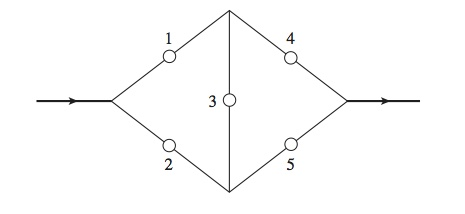
\includegraphics[width=\linewidth]{reliability}
    $s_i=1$ if functioning and $s_i=0$ if failed.\\
    $\Phi = 1 \Leftrightarrow$ overall system is functioning
    \begin{align*}
        &\Phi(s_1,s_2,s_3,s_4,s_5) = \max\{ s_1s_3s_5, s_2s_3s_4,s_2s_5,s_1s_4  \}\\
        &P(S_i=1)=p_i=1-P(S_i=0)\\
        &r(p_1, p_2, p_3, p_4, p_5) = P(\Phi=1) = E(\Phi)
    \end{align*}
    Using Antithetic Pairs
    \begin{enumerate}
        \item Generate $U_1, U_2, \cdots, U_5 \sim Unif(0,1)$
        \item Set $S_i = 1$ if $U_i\leq p_i$ else 0
        \item Compute $W_i=\Phi(S_1, \cdots, S_5)$
        \item Set $S_i' = 1$ if $1-U_i \leq p_i$ else 0
        \item Compute $W_i' = \Phi(S_1', \cdots, S_5')$
    \end{enumerate}

    \subsubsection{Specific Method for Normal}
    if $X\sim N(\mu, \sigma^2)$, then antithetic RV is $X'=2\mu-X$
    \begin{align*}
        X_i &= h(W_1, \cdots, W_d)\\
        X_i' &= h(2\mu_1-W_1, \cdots, 2\mu_d - W_d)
    \end{align*}

    \subsection{Control Variables}
    estimate $\mu = E(X)$, require $\mu_Y$ to be known
    \begin{align*}
        \hat\mu &=X + c^*(Y-\mu_Y)\\
        c^* &= - \frac{Cov(X,Y)}{Var(Y)}\\
        Var(X+c^*(Y-\mu_Y))&=Var(X)-\frac{[Cov(X,Y)]^2}{Var(Y)}
    \end{align*}
    Note: (var reduction / var(X) = corr(X,Y))
    \begin{align*}
        E(U) = \frac{1}{2}~&~E(U^2) = \frac{1}{3}\\
        \rho(X, Y)^2 &= \frac{[Cov(X,Y)]^2}{Var(Y)}\cdot\frac{1}{Var(X)}
    \end{align*}
    Using Control Variables in Simulation
    \begin{enumerate}
        \item Identify a RV $X$ and write a program to simulate it
        \item Generate $X_1, X_2, \cdots, X_n$
        \item Identify $Y_1, \cdots, Y_n$ that was part of the simulation with a known $\mu_Y$
        \item Estimate $\hat c^*$ from data
        \item Set $W_i = X_i + c^*(Y_i-\mu_Y)$
        \item Compute $\bar W = \frac{1}{n}\sum_{i=1}^n W_i$, and $s^2=\frac{1}{n-1}\sum_{i=1}^n(W_i-\bar W)^2$
        \item Then $(1-\alpha)100\%$ CI: $\bar W \pm z(\alpha/2)s/\sqrt{n}$
    \end{enumerate}
    
    \hl{Back to Example1: Integrating $e^x$}\\
    Using $U$ as control variate, $E(U)=0.5$\\ 
    $Var(e^U+c^*(U-1/2)) << Var(e^U)$\\
    use $X_i = e^U + c^*(U-1/2)$

    \hl{Back to Example2: Reliability Function}\\
    Using $Y=\sum_{i=1}^5 S_i$ as control variate, $E(Y)=E(\sum_{i=1}^5S_i)=\sum_{i=1}^np_i$\\
    use $X_i = W_i + c^*(Y_i-\sum_{i=1}^5 p_i)$

    \subsubsection{Var of estimator}
    \begin{tabular}{l @{ : } l}
        Control variables & $Var(W)$\\
        Antithetic pair & $Var(Y)$
    \end{tabular}

    \subsection{Importance Sampling}
    Importance sampling can be used more generally to reduce variance of estimator. 
    However, it is difficult to choose an alternative density to use as theoretical analysis is often difficult.

    \hl{Example3: Quality Control Studies}\\
    Let $X_1, X_2, \cdots$ be a sequence of i.i.d $N(\mu, 1)$ RV with $\mu<0$\\
    Wish to know when will partial sum exceed limits
    \begin{align*}
        S_n &= \sum_{i=1}^n X_i\\
        N &= \min\{n: S_n < -A \text{ or } S_n > B \}
    \end{align*}
    A, B are fixed known positive numbers, N is stopping time\\
    Interested in estimating $P(S_n > B)$\\
    Instead of $N(\mu, 1)$, consider $N(-\mu, 1)$ and estimate with $\bar W$
    \begin{align*}
        W_i &= I\left( \sum_{i=1}^N X_i > B  \right) \frac{\prod_{i=1}^N f_\mu(X_i)}{\prod_{i=1}^Nf_{-\mu}(X_i)}\\
        \because &\frac{f_\mu(x)}{f_{-\mu(x)}}=e^{2\mu x}\\
        \Rightarrow W_i &= I\left( \sum_{i=1}^N X_i > B  \right)exp(2\mu\sum_{i=1}^N X_i)
    \end{align*}

    \section{Statistical Validation Techniques}
    General step for hypothesis testing
    \begin{enumerate}
        \item Take note of assumption
        \item Specify $H_0, H_1$ and significant level $\alpha=0.05$
        \item Compute test statistics
        \item Obtain p-value of obs a more extreme test statistics
        \item State the conclusion (reject or do not reject $H_0$)
    \end{enumerate}

    \subsection{Goodness of Fit Tests: Discrete data}
    \begin{align*}
        H_0: P(Y_j=i)=p_i, i\in[0, K-1]
    \end{align*}
    Let $N_i:=$ number of $Y_j=i$\\
    For a fixed $i$
    \begin{align*}
        X_j = \begin{cases}
            1, Y_j = i\\
            0, Y \neq i
        \end{cases}
    \end{align*}
    $j\in[1, n]$. Then under $H_0, P(X_j=1)=P(Y_j=i)=p_i$
    \begin{align*}
        N_i = \sum_{j=1}^n X_j \sim Bin(n, p_i)
    \end{align*}
    Therefore, under $H_0$, $E(N_i)=np_i$. Using $(N_i-np_i)^2$ as indication for how likely our assumption is true

    \begin{align*}
        T = \sum_{i=0}^{K-1} \frac{(N_i-np_i)^2}{np_i} \sim\chi^2_{K-1}
    \end{align*}
    \begin{tabular}{l @{ := } l}
        $N_i$ & num of observation that took value $i$\\
        $p_i$ & postulated probability of observing the value $i$\\
        $n$ & num of obs we made  \\
        $K$ & num of different possible values $Y_i$ can take
    \end{tabular}

    When $n$ is large $(n\geq 50), T\sim \chi^2_{K-1}$\\
    When $n$ is small, use simulation to estimate the p-value

    \subsubsection{$\chi^2$ test summary}
    Summary of $\chi^2$ test when all parameters in $H_0$ are fully specified
    \begin{enumerate}
        \item independent set of $Y_1, \cdots, Y_n$ from real-life process
        \item $H_0: Y_1, \cdots, Y_n$ are from pmf $p_i$ and $H_1$ is not
        \item $T = \sum_{i=0}^{K-1}\frac{(N_i-np_i)^2}{np_i}\sim \chi^2_{K-1}$
        \item p-value is area under $\chi^2_{K-1}$ to the right of observed test stat
    \end{enumerate}

    \hl{Example 1 ($\chi^2$ Goodness of Fit test)}\\
    $H_0: p_i = 0.2, i\in[0, 4]$\\
    $N_i = \{12, 5, 19, 7, 7\}$, $E(N_i)=10$\\
    $T = (4+25+81+9+9)/10=12.8$\\
    $P_{H_0}(T\geq 12.8) = P(\chi^2_4\geq12.8)=0.0123$
		\begin{lstlisting}[language=R]
pchisq(12.8, df=4, lower.tail=FALSE)
        \end{lstlisting}

    \subsubsection{$\chi^2$ test after estimation of parameters}
    If pmf in $H_0$ is not completely specified and we need to estimate $m$ parameters
    \begin{align*}
        \chi^2_{K-1-m}
    \end{align*}

    \hl{Example 2 (Comparing to $Pois(\lambda)$ Distribution)}
    \begin{tabular}{l | l l l l l l}
        i & 0 & 1 & 2 & 3 & 4 & 5 or more\\
        \hline
        $N_i$ & 6 & 2 & 1 & 9 & 7 & 5\\
        \hline
        $\hat p_i$ & 0.05 & 0.1596 & 0.2312 & 0.2237 & 0.1622 & 0.1682\\
        \hline
    \end{tabular}
    \begin{enumerate}
        \item find $\hat\lambda=\frac{\sum_{i=1}^{30}Y_i}{30}=87/30$, $Y_i = N_i \cdot i$
        \item $T_{obs} = \sum_{i=0}^5\frac{(N_i - 30\hat p_i)^2}{30\hat p_i}=19.887$
        \item $P(\chi^2_{K-1-m=6-1-1=4}\geq19.887)=0.0005$
    \end{enumerate}

    \subsubsection{Estimating p-value by Simulation}
    \hl{Algorithm 1 (Estimating p-value in Goodness-of-fit Test)}
    \begin{enumerate}
        \item use observed data $Y_1, Y_2, \cdots, Y_n$ to compute the observed test statistics
            \begin{align*}
                T_{obs} &= \sum_{i=0}^{K-1}\frac{(N_i-np_i)^2}{np_i}
            \end{align*}
        \item For $s\in[1, M]$, M is the max iter
            \subitem[1] Generate $Y_1^s, Y_2^s, \cdots, Y_n^s$ from pmf $p_i$ in $H_0$
            \subitem[2] Compute $N_0^s, N_1^s, \cdots, N_{K-1}^s$ from $Y_1^s, \cdots, Y_n^s$
            \subitem[3] Compute $T_s = \sum_{i=0}^{K-1}\frac{(N_i^s-np_i)^2}{np_i}$
            \subitem[4] Set $V_s = I(T_s \geq T_{obs})$
        \item estimate p-value with \begin{align*} \bar V = \frac{1}{M}\sum_{s=0}^M V_s  \end{align*}
    \end{enumerate}

    \subsection{Goodness of Fit Tests: Continuous data}

    \subsubsection{Forming Discrete Data from Continuous}
    \begin{enumerate}
        \item Bin $Y_i$ into $K$ distinct intervals\\
            $(-\infty, y_1], (y_1, y_2], \cdots, (y_{K-1}, \infty)$
        \item Set $Y_i^d=i-1$ if $Y_j$ lies in interval $(y_{i-1}, y_i]$.\\
            Set up $N_i$ and test goodness of fit
        \item $H_0: P(Y_j^d=i)=F(Y_{i=1})-F(y_i), i\in[0, K-1]$
    \end{enumerate}

    \subsubsection{Kolmogorov Smirnov Test}
    where $y_{(j)}$ are the ascending ordered $Y_j$, $F_e$ is empirical cdf, $y:=F(x)$

    \begin{align*}
        F_e(x) &= \frac{\#i: Y_i\leq x}{n}\\
        D &= \max_x |F_e(x) - F(x)|\\
          &=\max\left\{ \frac{j}{n} - F(y_{(j)}), F(y_{(j)}) - \frac{j-1}{n}  \right\}, j \in[1, n]\\
        P_F(D\geq d) &=P_F\left( \max_{0\leq y \leq 1}|\frac{\#i:U_i \leq y}{n} - y| \geq d  \right)
    \end{align*}
    \hl{calculate $\max\left\{ \frac{j}{n} - F(y_{(j)}), F(y_{(j)}) - \frac{j-1}{n}  \right\}$}

    \begin{enumerate}
        \item get $F(y_i)$
        \item sort $F(y_i)$ ascending
        \item calculate $\max\left\{ \frac{j}{n} - F(y_{(j)}), F(y_{(j)}) - \frac{j-1}{n}  \right\}$
    \end{enumerate}

    \hl{Algorithm 2: Estimating p-value in KS test by simulation}\\
    For $s \in [1, M]$, $M:=$ number of iteration to run
    \begin{enumerate}
        \item Generate $U_1^{(s)}, U_2^{(s)}, \cdots, U_n^{(s)}$ i.i.d from unif(0,1)
        \item Compute \begin{align*}
                W_k = \max_{0\leq y \leq 1}|\frac{\#i:U_i \leq y}{n}-y|
            \end{align*}
        \item Set $V_s = I(W_k \geq D_{obs})$
    \end{enumerate}
    Estimate p-value with
    \begin{align*}
        \bar V = \frac{1}{M}\sum_{s=1}^M V_s
    \end{align*}
    Remember to sort the generated $U_i^{(s)}$

    \subsection{Two Sample Rank Sum Test}
    $X_1, \cdots, X_n, Y_1, \cdots, Y_m$, data from simulation and real world\\
    $H_0:$ $n+m$ values are iid
    \begin{enumerate}
        \item order $n+m$ values
        \item $R_i$ denote the rank of the $X_i$ among the $n+m$ valuse
        \item $R = \sum_{i=1}^nR_i$ as the test stat
        \item $X_i, Y_i$ from diff dist for extreme large or small $R$
        \item when $n, m$ are large
            \begin{align*}
                R&\sim N(\frac{n(n+m+1)}{2}, \frac{nm(n+m+1)}{12}\\
                \frac{R-\frac{n(n+m+1)}{2}}{\sqrt{\frac{nm(n+m+1)}{12}}}&\sim N(0,1)\\
                r^* &= \frac{r-\frac{n(n+m+1)}{2}}{\sqrt{\frac{(nm(n+m+1))}{12}}}\\
                \text{p-value} &= \begin{cases}
                    2P(Z < r^*) & r \leq n(n+m+1)/2\\
                    2P(Z>r^*) & r > n(n+m+1)/2
                \end{cases}
            \end{align*}
    \end{enumerate}
    Note: if tie, take average rank. Remember to c.c.

    \hl{Example 5 (Two Sample Rank Sum test)}
    $X = \{132, 104, 162, 171, 129\}$, $Y = \{107, 94, 136, 99, 114, 122, 108, 130, 106, 88  \}$
    $rank(X) = R_i = [12, 4, 14, 15, 10], R = \sum R_i = 55$\\
    p-value = $2P_{H_0}(R \geq 55) \approx 2P(Z\geq \frac{54.5-40}{\sqrt{50(16)/12}})$, cc

    \subsection{Validating Poisson Processes}

    \subsubsection{Nonhomogeneous Poisson Process}
    $N_i :=$ num of arrivals on day $i$
    \begin{align*}
        N_i \sim Pois(m(T))\\
        m(T) = \int_0^T\lambda(s) ds
    \end{align*}
    Then using $E(N_i)$ and goodness of fit test

    \subsubsection{Homogenous Poisson Process}
    Key assumption to test, where $T$ is the total time interval
    \begin{align*}
        H_0:& \text{ arrival time  } \sim unif(0, T)\\
        H_1:& \text{ not uniform }
    \end{align*}
    Note: it's arrival time and not inter-arrival time (which follow exp dist)

\section{Quick tips}
\subsection{Easiest way to generate RV}
\begin{tabular}{l @{ : } l}
    Ber & $u\sim unif(0,1)$, set $X=1$ if $u\geq p$ else $0$\\
    Binom & generate $n$ Ber with $p$\\
    Pois Process & homogeneous, thining method\\
    Exp & numeric inversion $X=-\frac{1}{\lambda}log(u)$\\
    Gamma & generate $\alpha$ Exp with $\lambda$\\
    Normal & Box-Muller transformation with $u_1, u_2$
\end{tabular}
\subsection{Finding simulation algo cdf}
Use $P(Y\leq y \cap U \geq p)$ instead of conditional probability


\end{multicols}
\end{document}
